\documentclass{article}
\usepackage{tikz}
\usepackage[utf8]{inputenc}
\usepackage{ amssymb }
\usepackage{amsfonts}
\usetikzlibrary{automata,positioning,arrows}

\title{Programación Avanzada . Tarea 6}
\author{Fabián Romero Jiménez}
\begin{document}
\maketitle
\begin{enumerate}


\item[\bf{Abstract Factory.}]
\begin{itemize}
\item{Descripción}\\

Proporciona una interfaz para crear familias de objetos o que dependen entre sí, sin especificar sus clases concretas.\\
La idea detrás del patron Abstract Factory (que en español se traduciría como fabrica abstracta) consiste en la noción de que nuestro programa (o el cliente de una clase que nosotros proporcionamos) trabaja con una serie de productos (como los de una fábrica) que tienen unas determinadas características (por ejemplo tenemos productos embotellados y productos en tetrabrick). Nuestro programa va a utilizar dichos productos realizando una serie de acciones sobre ellos (como meter las botellas en unos camiones y los tetrabricks en otros) sin importarle quien le está suministrando los productos.\\
Así mismo existen una serie de fábricas que producen esos productos que vamos a tratar, una fábrica fabrica cocacola y otra pepsi pero ambas en botellas de las que nuestro programa trata. Al final, el concepto básico consiste en que a nuestro programa (o cliente) no le importa lo que haya dentro de la botella ni quien lo haya producido mientras sea una botella.
Desde el punto de vista software el ejemplo anterior se traduce en una situación en la que nuestro programa maneja un tipo de objetos con unas características comunes y algunas caracterísiticas propias. Esto en general en software se resuelve mediante el uso de dos características de los lenguajes de programación orientados a objetos, las clases abstractas y los interfaces.\\

\item{Problema}\\

El patrón de diseño Abstract Factory aborda el problema de la creación de familias de objetos (como por ejemplo iterfaces gráficos) que comparten toda una serie de características comunes en los objetos que componen dichas familias.

\item{Aplicabilidad}\\

El uso de este patrón está recomendado para situaciones en las que tenemos una familia de productos concretos y prevemos la inclusión de distintas familias de productos en un futuro.

\item{Estructura}\\
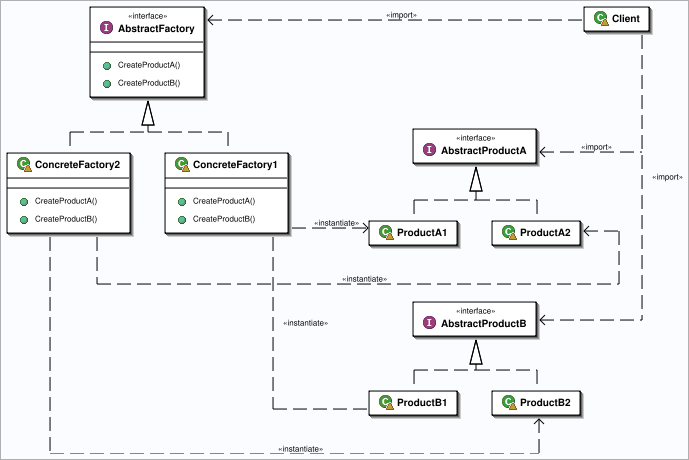
\includegraphics[width=12cm]{abstract.png}

De esta forma nuestro programa realiza unas ciertas operaciones sobre dichas características comunes sin importarle que otras características tenga el objeto en cuestión. Por otro lado existen distintos productores de dichos objetos. Un ejemplo muy típico en muchos frameworks de programación que sigue este patrón se da en el caso de las familias de interfaces gráficos. Así existen diversas fábricas de interfaces que proporcionan sus propios botones, campos de texto, listas desplegables, etc... Todas ellas basadas en los tipos básicos. Los clientes obtienen una familia y proceden a utilizar los controles usando el tipo abstracto genérico que da soporte.

\item{Aplicaciones reales}\\
Un caso bastante común es el similar al presentado en el ejemplo de código, es decir, una familia de algoritmos de comunicación por distintos medios que permiten el envio de información entre pares (por ejemplo). De esta forma nuestro programa puede usar comunicación TCP, UDP o cualquier otro protocolo que se nos ocurra sobre un dispositivo no estandar o que no soporte IP.
Interfaces gráficos
Otro caso relativamente común de uso de este patrón se da en la creación de familias de interfaces gráficos en las cuales los elementos (productos) del interfaz se mantienen constantes (por ejemplo labels, botones, cajas de texto ...) pero el dibujado de dichos elementos puede delegarse en distintas familias (por ejemplo QT, GTK, etc) de forma que, en función de la fábrica seleccionada obtenemos unos botones u otros.


\item[\bf{Builder.}]

\begin{itemize}
\item{Descripción}\\

Separa la construcción de un objeto complejo de su representación, de forma que el mismo proceso de construcción pueda crear diferentes representaciones.
Permite a un objeto (fuente) construir un objeto complejo especificando sólo su tipo. El objeto constructor (fuente) se compone de una serie de partes que individualmente van formando el objeto complejo. Así se abstrae el proceso de creación del objeto complejo para que se puedan crear representaciones diferentes con el mismo proceso. 
Se nos pueden ocurrir muchos ejemplos para el patrón Builder, vehículos, recetas, electrodomésticos y cualquier cosa que esté compuesta por muchas partes. También se utiliza mucho para crear los objetos del patrón Composite (patrón estructural). El siguiente ejemplo va ensamblando los componentes de un ordenador según el uso que le queramos dar. 
El patrón constructor sigue la misma idea que el patrón factoría, pero no se encarga simplemente de devolver una clase, si no de construir una composición de objetos entera, por compleja o sencilla que sea. El caso más habitual es el de construir una interfaz de usuario, pero no se limita únicamente a componentes visuales.

\item{Intención}\\

Separar la construcción de un objeto complejo de su representación de modo que el mismo proceso de construcción pueda crear diferentes representaciones.

\item{Motivación}\\

Los objetos que dependen de un algoritmo tendrán que cambiar cuando el algoritmo cambia. Por lo tanto los algoritmos que estén expuestos a dicho cambio deberían ser separados, permitiendo de esta manera reutilizar algoritmos para crear diferentes representaciones.

\item{Usos}\\

El algoritmo para creación de un objeto complejo debe ser independiente de las partes que conforman el objeto y cómo están ensambladas.\\

El proceso de construcción debe permitir diferentes representaciones del objeto que se construye.

\item{Estructura}\\
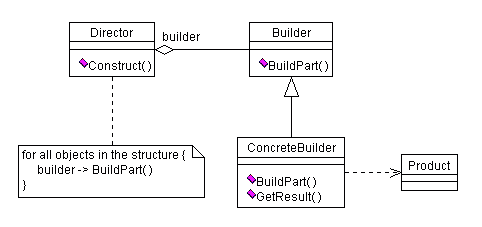
\includegraphics[width=12cm]{builder.png}


\item{Consecuencias}\\
Permite variar la representación interna de un producto.\\
Permite separar el código de la construcción y la representación.\\
Da control refinado sobre el proceso de construcción.\\
\end{itemize}


\item[\bf{Iterator}]

\begin{itemize}
\item{Descripción}\\

Proporciona un modo de acceder secuencialmente a los elementos de un objeto agregado sin exponer su representación interna. El patrón de diseño Iterator tiene como finalidad proveer un camino para acceder a los elementos de una colección secuencial de objetos sin exponer la representación interna de dicho recorrido.
Una colección de objetos, tal como una lista deberían proveer una forma o camino de acceso a sus elementos sin exponer su representación interna.
Por otra parte, se podría necesitar también recorrer la lista de diferentes formas, dependiendo del problema al que se le deba dar solución. Pero probablemente no se quiera llenar la “interfase Lista” con operaciones que recorran sus elementos en distintas direcciones. También se podría tener más de un recorrido pendiente por recorrer en la misma lista.

El patrón Iterator  permite resolver los problemas anteriormente planteados. La idea principal de este patrón es tomar la responsabilidad de acceso y recorrido de los objetos de una lista, agregando a esta última un objeto de tipo Iterator.

La Clase Iterator define una interfase que permite acceder a los elementos de una lista. Un Objeto de tipo Iterator es el encargado de ir guardando el recorrido del elemento corriente, es decir, conoce los elementos que ya se han recorrido.
Por ejemplo, una clase List necesitaría una clase ListIterator con la siguiente relación entre ellas. 

Antes de instanciar la clase ListIterator se deberá proporcionar la lista de los elementos a recorrer. Una vez instanciada la clase ListIterator, se podrá tener acceso a los elementos de List, secuencialmente. La operación CurrentItem() (Item corriente), retorna el elemento corriente de la lista. Firts() inicializa el elemento corriente con el primer elemento de la lista, Next() avanza el elemento corriente a siguiente elemento de la lista y la operación IsDone() chequea que no se haya avanzado más allá del último elemento, es decir, chequea que el recorrido no haya finalizado.

Separando los mecanismos de recorrido de los objetos de la clase List permitirá definir  iteradores con diferentes políticas de recorrido, sin enumerarlos dentro de la interface List.

Por ejemplo la operación FilteringListIterator permitirá el acceso sólo a aquellos elementos de la lista que cumplan alguna restricción que actuará como filtro.

Es importante notar que la lista y el iterador están asociados, y que el cliente debe conocer que esta lista podrá ser recorrida de forma diferente a otras colecciones de objetos. Además el cliente debe optar por un tipo de objetos en particular. Sería mucho mejor si se pudiera cambiar el tipo de los elementos de la lista sin necesidad de cambiar el código del cliente que la utiliza. Esto puede lograrse generalizando el concepto de iterador de manera tal que pueda soportar iteraciones polimórficas. Está ultima es una de las principales ventajas de utilizar el patrón de diseño Iterator

Como ejemplo, supongamos que tenemos una implementación especial de lista llamada SkipList. Estas listas especiales son estructuras de datos probabilísticas con características similares a los árboles balanceados. Por lo tanto deberemos definir un iterador que funcione para ambos tipos de listas. 

\item{Ejemplo de aplicación del patrón  Iterator}\\

 Para llevar este objetivo a cabo, se define una clase AbstractList que provee una interface común para la manipulación de listas. De la misma manera, se necesitará una clase abstracta Iterator que defina una interface común de iteración. Luego se define una subclase concreta de la interface Iterator para las diferentes implementaciones de lista. Como resultado de esto, el mecanismo de recorrido será independiente del tipo concreto de la colección de objetos.  

\item{Aplicabilidad}\\

 El problema siguiente es cómo crear un iterador. Para ello se debe escribir el código sin tener en cuenta el tipo específico de los elementos de la lista a recorrer motivo por el cual no se podrá instanciar  una lista de un tipo particular. Como solución a esto se propone que los objetos de la lista tomen la responsabilidad de crear sus propios iteradores. Esto requiere una operación adicional, llamada CreateIterator() a través de la cual el cliente pueda solicitar un objeto iterador.
Es conveniente utilizar el patrón Iterador en las siguientes situaciones:
\begin{enumerate}
\item	Para acceder al contenido de colecciones de objetos sin exponer la representación interna del recorrido realizado
\item	Para soportar diferentes recorridos sobre la misma colección de objetos 
\item	Para proveer una interfaz común de recorrido de diferentes colecciones de objetos (iteración polimórfica).
Participantes 
 Estructura del patrón Iterator
\item	Iterator: define una interface de acceso y recorrido de los elementos de una lista.
\item	ConcreteIterator: implementa la interface Iterator y mantiene o guarda el recorrido del ítem corriente
\item	Aggregate: (colección) define una interface que permite crear objetos de tipo Iterator. 
\item	ConcreteAggregate: implementa la interface de creación de objetos Iterator y retorna una instancia apropiada de la clase ConcreteIterator
\end{enumerate}

\item{Colaboraciones}\\

Un ConcreteIterator mantiene la pista de cuales fueron los objetos que se recorrieron y conoce el elemento siguiente al actual. 


\item{Consecuencias}\\

Este patrón tiene tres consecuencias importantes:  

\begin{enumerate}
\item	Soporta  variaciones en el recorrido de una colección, puesto que estructuras complejas pueden requerir recorridos en muchas formas. Los iteradores hacen fácil cambiar el algoritmo de recorrido, con sólo reemplazar la instancia del iterador a una diferente.
\item	Los iteradores simplifican la interfaz de las colecciones, ya que la interfaz de los recorridos se encuentra en los iteradores y no en la clase que corresponde a la estructura en cuestión.
\item	Más de un recorrido puede estar pendiente en una colección, puesto que cada iterador mantiene la pista de su recorrido. Por lo tanto, se puede tener más de un recorrido en progreso al mismo tiempo.
\end{enumerate} 

\item{Estructura}\\
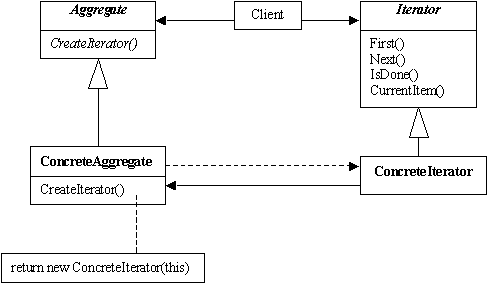
\includegraphics[width=12cm]{iterator.png}


\item{Implementaciones}\\

Los iteradores tienen muchas variantes y alternativas en cuanto a la implementación. Las ventajas dependen de las estructuras de control que el lenguaje provea. Algunas de las más importantes son las siguientes.
\begin{enumerate}
\item	¿Quién controla la iteración?
La iteración puede ser controlada de forma interna (controlada por el iterador), o de forma externa (controlada por el cliente).
\item	¿Quién define el algoritmo de recorrido?
El algoritmo puede ser definido dentro de la colección, con lo cual el iterador es utilizado sólo como cursor de la posición actual o en la clase Iterator
\item	Operaciones adicionales en el iterador
Se pueden adicionar operaciones a las ya básicas (First, Next, IsDone y CurrentItem)
\item	Iteradores para tipos compuestos (Composite)
\item	Iteradores nulos
Referido a un iterador útil para el manejo de condiciones de frontera.
\end{enumerate}
\end{itemize}



\item[\bf{Template Method}]
\begin{itemize}
\item{Descripción}\\

Define en una operación el esqueleto de un algoritmo, delegando en las subclases algunos de sus pasos. Permite que las subclases redefinan ciertos pasos del algoritmo sin cambiar su estructura.
Define en una operación el esqueleto de un algoritmo, delegando en las subclases algunos de sus pasos, esto permite que las subclases redefinan ciertos pasos de un algoritmo sin cambiar su estructura.
Un Template Method es un patrón de diseño el cual define una estructura algorítmica en la súper clase, delegando la implementación a las subclases. Es decir, define una serie de pasos, en donde los pasos serán redefinidos en las subclases.

\item{Proposito}\\

Usando el Template Method, se define una estructura de herencia en la cual la superclase sirve de plantilla (”Template” significa plantilla) de los métodos en las subclases. Una de las ventajas de este método es que evita la repetición de código, por tanto la aparición de errores.

\item{¿Cuándo Usarlo?}\\

Este patrón se vuelve de especial utilidad cuando es necesario realizar un algoritmo que sea común para muchas clases, pero con pequeñas variaciones entre una y otras.


\item{Estructura}\\
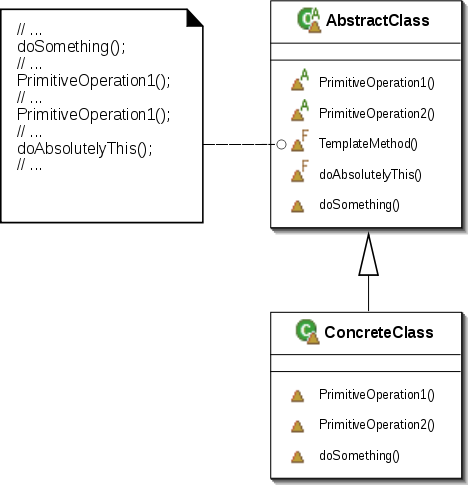
\includegraphics[width=12cm]{Template_Method.png}
\end{itemize}

\item[\bf{Mediator}]
\begin{itemize}
\item{Descripción}\\

Define un objeto que encapsula cómo interactúan un conjunto de objetos. Promueve un bajo acoplamiento al evitar que los objetos se refieran unos a otros explícitamente, y permite variar la interacción entre ellos de forma independiente.
Define un objeto que coordine la comunicación entre objetos de distintas clases, pero que funcionan como un conjunto.
Un Mediator (o patrón de diseño) coordina las relaciones entre sus asociados. Permite la interacción de varios objetos, sin generar acoples fuertes en esas relaciones.

\item{Motivación}\\

Cuando muchos objetos interactúan con otros objetos, se puede formar una estructura muy compleja, con objetos con muchas conexiones con otros objetos. En un caso extremo cada objeto puede conocer a todos los demás objetos. Para evitar esto el patrón Mediator encapsula el comportamiento de todo un conjunto de objetos en un solo objeto.

\item{Aplicabilidad}\\

Usar el patrón Mediator cuando:

\begin{enumerate}
\item Un conjunto grande de objetos se comunica de una forma bien definida, pero compleja.
\item Reusar un objeto se hace difícil por que se relaciona con muchos objetos.
\item El comportamiento de muchos objetos que esta distribuido entre varias clases, puede resumirse en una o varias por subclasificacion.
\end{enumerate}

\item{Estructura}\\
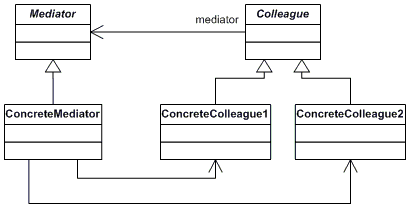
\includegraphics[width=12cm]{mediator.png}


\end{itemize} 
\end{itemize}
\end{enumerate}


\end{document}  
